\documentclass[../main.tex]{subfiles}

\begin{document}

\section{Comentaciones de puentes y estribos}
\subsection{Introducción}

Los puentes son quizás las obras de ingeniería más funcionales. Deben armonizar
con su entorno y puede necesitar cumplir varias funciones, tales como ser un 
cruce de un río en un paisaje rural como un viaducto dentro de una zona urbana.

Para su realización se hacen estudios tecnico económicos que cada vez llevan a 
estructuras de mayor luz. Estos diseños concentran en pocos elementos estrucutrales
grandes cargas verticales, esfuerzos horizontales y momentos, que deben ser 
trasmitidos al suelo de fundación.

\subsection{Elección de tipo de cimentación para puentes}


\subsubsection{Cimentaciones de puentes situados en agua}

Se utilizan varios métodos especiales de construcción, como:

\begin{itemize}
  \item Adecuados a los agentes naturales adversos.
  \item Deben resistir socavaciones que se producirán al paso de las grandes
    corrientes.
  \item Deben resistir la agresividad del agua a los hormigones.
\end{itemize}

En cuanto a una elección general, se deberán establecer condiciones según varios
aspectos partículares de la obra. Es importante hacer un estudio exhaustivo tanto
en obras grandes como en obras de pequeña envergadura que pueden tener grandes
problemas de socavación o erosión, debido a bajos caudales en estiaje y grandes
caudales en crecidas. 

\subsection*{Diferentes soluciones para cimentaciones de puentes}
\subsection{Cimentaciones por escollera}

Es un procedimiento empleado en la antiguedad para aumentar un sobrenivel. Su 
principal inconveniente radica en el gran obstáculo que esta plataforma crea al
paso de la corriente, lo que conduce a un aumento de la velocidad del agua y una
posible socavación, que puede perjudicar al puente.

\begin{figure}[ht]
  \centering
  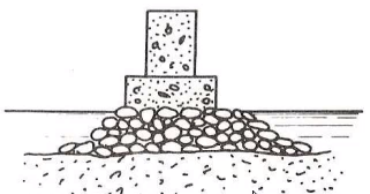
\includegraphics[width=0.5\textwidth]{../images/20210419/escollera}
  \caption{Cimentación sobre escollera}
  \label{fig:escollera}
\end{figure}

\subsubsection{Cimentaciones directas a cielo abierto}

\textbf{Ataguías}

Es otra forma de cimentar, creando un recinto con ataguías que genera una
estanquidad para la construcción, como se muestra en \Cref{fig:ataguia}

El material debe elegirse cuidadosamente, disponiendo al menos un núcleo central
con material arcilloso impereable y protegido el talud aguas arriba con material
rocoso.

\begin{figure}[htpb]
  \centering
  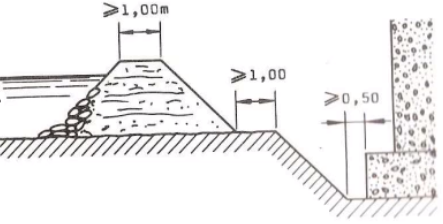
\includegraphics[width=0.8\textwidth]{../images/20210419/ataguia}
  \caption{Esquema de ataguia}
  \label{fig:ataguia}
\end{figure}

Se debe construir con una revancha de $\SI{0.3}{m}$ a $\SI{0.5}{m}$ con relación
al máximo caudal esperado.

También sirve para desvios parciales de ríos. Además, cuando el terreno del 
fondo es permeable o tiene grandes calados, es posible lograr un recinto estanco
mediante el hincado de \textbf{tablaestacas metálicas} hasta el terreno impermeable.

Otros defectos de estanqueidad se pueden resolver desde la propia excavación
mediante el relleno de juntas con inyecciones de mortero. Es importante saber que 
\textit{no pueden evitarse todas las filtraciones}, por lo que existen distintos
sistemas, tales como pueden ser cunetas para luego ser bombeadas, o en caso de
estar sobre piedra pueden usarse cajones de fondo abierto metálicos.

Estos cajones nos permiten crear recintos estancos con fondos permeables donde se 
puede hormigonar, como en \Cref{fig:ataguia-cajon}

\begin{figure}[htpb]
  \centering
  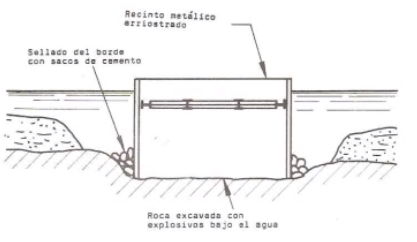
\includegraphics[width=0.8\textwidth]{../images/20210419/ataguia-cajon}
  \caption{Esquema de cajón abierto}
  \label{fig:ataguia-cajon}
\end{figure}    

\textbf{Ataguias de doble pared}

Con grandes calados, se pueden utilizar este tipo de sistema, que permiten crear
mayores espesores de ataguía que permiten crear espacios estancos. 

\begin{figure}[h]
  \centering
  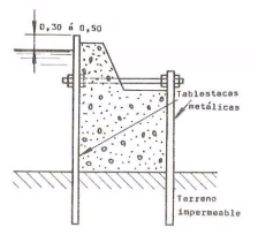
\includegraphics[width=0.5\textwidth]{../images/20210419/ataguia-doble}
  \caption{Esquema de ataguía de doble pared}
  \label{fig:ataguia-doble}
\end{figure}

Por último, se pueden utilizar ataguías celulares para grandes calados. En general,
cada solución es única para cada problema, por la diversidad de las condiciones 
del terreno de fundación.

\subsection{Cimentaciones con pilotes}

\subsubsection{Pilotes in-situ}

Cuando el terreno resistente no resulta fácilmente accesible, pueden utilizarse
pilotes como cimentación profunda. Si el elemento será situado en agua, primero
deberá disponerse de una plataforma de trabajo adecuada para poder ejecutar los
pilotes.

Si el calado es pequeño, se pueden construir \textit{terraplesnes provicionales},
que establecen una plataforma de trabajo por encima del nivel de agua permitiendo
la construcción de pilotes como si fuera en tierra. Incluso se puede crear un
recinto estanco mediante la utilización de tablaestacas, como se ve en \Cref{fig:terraplen-estanco}

\begin{figure}[htpb]
  \centering
  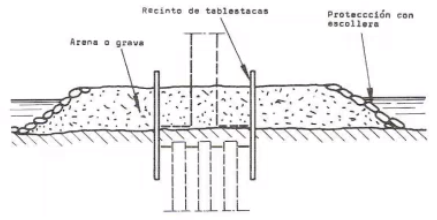
\includegraphics[width=0.8\textwidth]{../images/20210419/terraplen-estanco}
  \caption{Esquema de terraplen con tablaestacado.}
  \label{fig:terraplen-estanco}
\end{figure}

\subsubsection{Pilotes de madera}

Es principalmente un antecedente histórico, como los puentes usados en el Siglo
XVIII, que aún están en servicio. 

\subsubsection{Pilotes de hormigón}

En general no suelen ser utilizados los prefrabricaos. En cambio, es normal la 
utilzación de \textbf{pilotes pretensados de hormigón}, que permiten una mayor
resistencia. 

\subsubsection{Cabezales}

Son necesario para los \textbf{pilotes}, lo que produce las mismas dificultades
que en el caso de las zapatas directas construidas a un nivel inferior del río.

Si los pilotes son de gran diámetro, pueden ser prolognados en algunos casos hacía
arriba, sustituyendo a pilas y estribos y suprimiendo cabezales, lo que se llama
\textbf{pilotes columna}.

Si la zapata puede quedar por encima del río, se puede construir encima de la 
plataforma creada para la hinca de pilotes, y si se debe construir a nivel inferior
al del agua, se debe recurrir a un recinto impermeable provicional como los que
se describibieron, que tienen como objetivo contener laterlamente el hormigón
sumergido que permita el trabajo posterior seco.

Un tipo de alternativa es el uso de una \textbf{pila-cajón}, donde se conectaran
las pilas hasta donde se ejecutaron los pilotes, como se ve en \Cref{fig:pila-cajon}

\begin{figure}[ht]
  \centering
  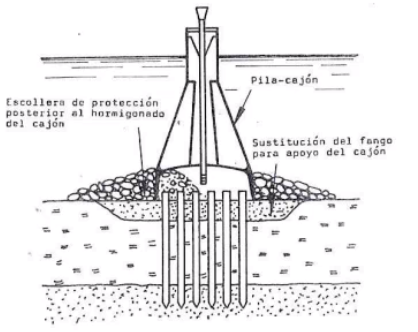
\includegraphics[width=0.6\textwidth]{../images/20210419/pila-cajon}
  \caption{Pila cajón usado en puente sobre Tage}
  \label{fig:pila-cajon}
\end{figure}

\subsection{Cimentaciones con cajón}

Podemos distinguir tres tipos:

\begin{itemize}
  \item Cajones con fondo abierto.
  \item Cajones de una sola celula.
  \item Cajones excavados con airea comprimido
\end{itemize}

%COMPLETAR

\subsubsection{Cajones con fondo abierto}

Se utilzados como se muestra en la \Cref{fig:cajon-abierto}, que permiten crear
una plataforma donde se puede realizar el hincado de los pilotes.

\begin{figure}[ht]
  \centering
  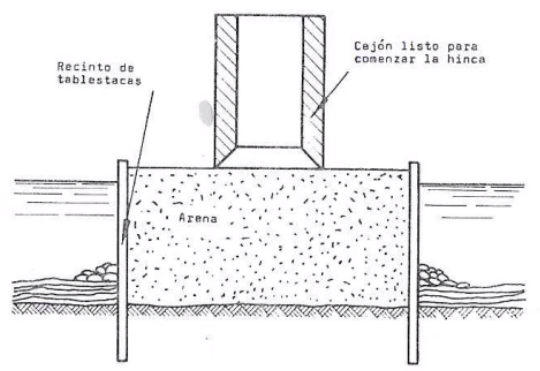
\includegraphics[width=0.8\textwidth]{../images/20210419/cajon-abierto}
  \caption{Cajón abierto}
  \label{fig:cajon-abierto}
\end{figure}

En algunos casos incluso se pueden llevar a partir de la flotación, y luego que
sea fondeado en la posición requerida.

%COMPLETAR

\subsubsection{Cajones excavados con aire comprimido}

Se usa cuando tenemos terrenos permeables o muy flojos, que pueden hacer que no 
sea posible la excavación en seco debido a posibles sifnamientos. 

Se puede recurrir a la excavación de un cajón auxiliandose con aire comprimido
para expulsar el agua del recinto del cajón.

Este proceso tiene tres fases, como se ve en la \Cref{fig:cajon-aire}. Este método
permite vencer obstáculos como estratos de roca intermedios u otros. Sin embargo,
solo es posible utilizarlo hasta unos $\SI{35}{m}$ de profundidad por lo que no 
es usable en la mayoría de los puentes.

\begin{figure}[ht]
  \centering
  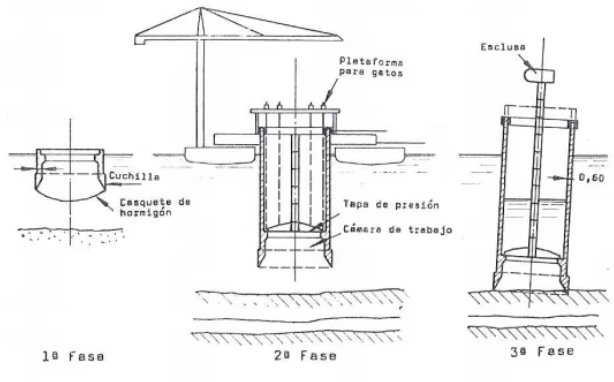
\includegraphics[width=0.8\textwidth]{../images/20210419/cajon-aire}
  \caption{Fases de un cajón con aire comprimido}
  \label{fig:cajon-aire}
\end{figure}

\subsubsection{Cajon con fondo}

Son un tipo de pila cajón que puede ser traido flotando, que son llenados con agua
para poder fondearlos.

\subsubsection{Cimentaciones por recintos mixtos}

En cimentaciones en tierra o isla artifical es posible ejecutar un recinto
poligonal, con módulos de pantalla que permiten ser excavados interiormente. 

El recinto exterior puede ser construido por pilotes tubulares metálicos hincados 
uno al lado del otro y ensamblados para permitir crear un recinto estanco.


\end{document}
